\documentclass[a4paper,12pt,twoside]{../includes/ThesisStyle}
\usepackage[utf8]{inputenc}
\usepackage[T1]{fontenc}

\usepackage[left=1.5in,right=1.3in,top=1.1in,bottom=1.1in,includefoot,includehead,headheight=13.6pt]{geometry}\renewcommand{\baselinestretch}{1.05}


% =============================================================================
%\usepackage[sectionbib]{chapterbib}	% Cross-reference package (Natural BiB)
%\usepackage{bibunits}
%\usepackage{natbib}					% Put References at the end of each chapter
\usepackage{algorithm}
\usepackage{alltt}
\usepackage{amsfonts}
\usepackage{amsmath}
\usepackage{amssymb}
\usepackage{cite}
\usepackage{color}
\usepackage{enumerate}
\usepackage{booktabs} % used for \midrule
\usepackage{fancyhdr}					% Fancy Header and Footer
\usepackage{graphicx}
\usepackage{ifthen}
\usepackage{latexsym}
\usepackage{multirow}
\usepackage{rotating}					% Sideways of figures & tables
\usepackage{stmaryrd}
\usepackage{subfigure}
\usepackage{url}         
\usepackage{xspace}
\usepackage[normalem]{ulem} % for \sout
\usepackage{xcolor}
\usepackage{tablefootnote}
\usepackage{pifont}

% =============================================================================

% Table of contents for each chapter
\usepackage[nottoc, notlof, notlot]{tocbibind}
\usepackage{minitoc}
\setcounter{minitocdepth}{1}
\mtcindent=15pt

\setcounter{secnumdepth}{3}
\setcounter{tocdepth}{2}
  
% =============================================================================
% Fancy Header Style Options

\pagestyle{fancy}                       % Sets fancy header and footer
\fancyfoot{}                            % Delete current footer settings

%\renewcommand{\chaptermark}[1]{         % Lower Case Chapter marker style
%  \markboth{\chaptername\ \thechapter.\ #1}}{}} %

%\renewcommand{\sectionmark}[1]{         % Lower case Section marker style
%  \markright{\thesection.\ #1}}         %

\fancyhead[LE,RO]{\bfseries\thepage}    % Page number (boldface) in left on even
% pages and right on odd pages
\fancyhead[RE]{\bfseries\nouppercase{\leftmark}}      % Chapter in the right on even pages
\fancyhead[LO]{\bfseries\nouppercase{\rightmark}}     % Section in the left on odd pages

\let\headruleORIG\headrule
\renewcommand{\headrule}{\color{black} \headruleORIG}
\renewcommand{\headrulewidth}{1.0pt}
\usepackage{colortbl}
\arrayrulecolor{black}

\fancypagestyle{plain}{
  \fancyhead{}
  \fancyfoot{}
  \renewcommand{\headrulewidth}{0pt}
}


% =============================================================================
% Clear Header Style on the Last Empty Odd pages
\makeatletter

\def\cleardoublepage{\clearpage\if@twoside \ifodd\c@page\else%
  \hbox{}%
  \thispagestyle{empty}%              % Empty header styles
  \newpage%
  \if@twocolumn\hbox{}\newpage\fi\fi\fi}

\makeatother

\newenvironment{maxime}[1]
{
\vspace*{0cm}
\hfill
\begin{minipage}{0.5\textwidth}%
%\rule[0.5ex]{\textwidth}{0.1mm}\\%
\hrulefill $\:$ {\bf #1}\\
%\vspace*{-0.25cm}
\it 
}%
{%

\hrulefill
\vspace*{0.5cm}%
\end{minipage}
}

\let\minitocORIG\minitoc
\renewcommand{\minitoc}{\minitocORIG \vspace{1.5em}}


\renewcommand{\epsilon}{\varepsilon}

% centered page environment
\newenvironment{vcenterpage}
	{\newpage\vspace*{\fill}\thispagestyle{empty}\renewcommand{\headrulewidth}{0pt}}
	{\vspace*{\fill}}
	

%=============================================================================

\usepackage{needspace}
\newcommand{\needlines}[1]{\Needspace{#1\baselineskip}}

\usepackage{xcolor}
\definecolor{source}{gray}{0.95}
% source code formatting
\usepackage{listings}
    % global settings for source code listing package
\lstset{
    basicstyle=\ttfamily\small,
    showspaces=false,
    showstringspaces=false,
    captionpos=b, 
    columns=fullflexible}

\lstdefinelanguage{ST}{
    keywordsprefix=\#,
    morekeywords=[0]{true,false,nil},
    morekeywords=[1]{self,super,thisContext},
    morekeywords=[2]{ifTrue:,ifFalse:,whileTrue:,whileFalse:,and:,or:,xor:,not:,by:,timesRepeat:},
    sensitive=true,
    morecomment=[s]{"}{"},
    morestring=[d]',
    escapechar={!},
    alsoletter={., :, -, =, +, <},
    moredelim=**[is][\itshape]{/+}{+/},
    literate=
        {^}{{$\uparrow$}}1
        {:=}{{$\leftarrow$}}1
        {~}{{$\sim$}}1
        {-}{{\sf -\hspace{-0.13em}-}}1  % the goal is to make - the same width as +
        {+}{\raisebox{0.08ex}{+}}1		% and to raise + off the baseline to match V
        , % Don't forget the comma at the end!
    style=STStyle
}
\lstdefinestyle{STStyle}{
    tabsize=4,
    %frame=leftline,
    % frame=bl,
    %framerule=2pt,
    %rulecolor=\color{gray},
    % backgroundcolor=\color{white},
    %backgroundcolor=\usebeamercolor[bg]{listing},
    basicstyle=\ttfamily\small,
    keywordstyle=\bf\ttfamily,
    % stringstyle=\color{orange},
    stringstyle=\mdseries\slshape,
    commentstyle=\it\rmfamily\color{darkgray}, 
    commentstyle=\mdseries\slshape\color{gray},
    %commentstyle=\mdseries\slshape,
    emphstyle=\bf\ttfamily,
    escapeinside={!}{!},
	%backgroundcolor=\color{source},
    %emphstyle={[2]\color{red}},
    %emphstyle={[3]\color{blue}\bf},
    %emphstyle={[4]\color{blue}},
    keepspaces=true
} 

%\lstnewenvironment{javacode}  [1][]{\lstset{language=java,#1}\needlines{#2}}{} 
%\lstnewenvironment{pythoncode}[2][]{\lstset{language=python,#1}\needlines{#2}}{}
\lstnewenvironment{stcode}    [2][]{\lstset{language=ST,#1}\needlines{#2}}{}
\lstnewenvironment{ccode}     [2][]
    {\lstset{language=C,numbers=left,escapechar=\$,numberstyle=\tiny,#1}\needlines{#2}}{}

% ON: I tried to pass the line number options in as arg #1 but it does not work for me
% I also could net get the line numbers to consistently increase
\lstnewenvironment{numstcode} [2][]
    {\lstset{language=ST,numbers=left,numberstyle=\tiny,numbersep=2pt,#1}\needlines{#2}}{}
\lstnewenvironment{numstcodecont} [2][]
    {\lstset{language=ST,numbers=left,numberstyle=\tiny,numbersep=2pt,firstnumber=last#1}\needlines{#2}}{}

\newcommand{\lst}[1]{{\tt #1}}

% In-line code (literal)

% In-line code (latex enabled)
% Use this only in special situations where \ct does not work
% (within Section headings ...):
\newcommand{\lct}[1]{{\textsf{\textup{#1}}}}
% Code environments
\lstnewenvironment{code}{%
	\lstset{%
		% frame=lines,
		frame=single,
		framerule=0pt,
		mathescape=false
	}
}{}

%\renewcommand{\lstlistingname}{Code Example}

% =============================================================================
\newboolean{showcomments}
\setboolean{showcomments}{true}

\ifthenelse{\boolean{showcomments}} {
	\newcommand{\ugh}[1] {\textcolor{red}{\uwave{#1}}}	% please rephrase
	\newcommand{\ins}[1] {\textcolor{blue}{\uline{#1}}}	% please insert
	\newcommand{\del}[1] {\textcolor{red}{\sout{#1}}}	% please delete
	\newcommand{\chg}[2] {								% please change
		\textcolor{red}{\sout{#1}}{\ra}
		\textcolor{blue}{\uline{#2}}}
	\newcommand{\nbc}[3]{								% comment
		{\colorbox{#3}{\bfseries\sffamily\scriptsize\textcolor{white}{#1}}}
		{\textcolor{#3}{\sf\small$\blacktriangleright$\textit{#2}$\blacktriangleleft$}}}

}{
	\newcommand{\ugh}[1]{#1}							% please rephrase
	\newcommand{\ins}[1]{#1}							% please insert
	\newcommand{\del}[1]{}								% please delete
	\newcommand{\chg}[2]{#2}							% please change
	\newcommand{\nbc}[3]{}								% comment
}

% =============================================================================
\usepackage[pagebackref,hyperindex=true]{hyperref}


% Links in pdf
\usepackage{color}
\definecolor{linkcol}{rgb}{0.0, 0.0, 0.0} 
\definecolor{citecol}{rgb}{0.0, 0.0, 0.0} 

% Change this to change the informations included in the pdf file
% See hyperref documentation for information on those parameters
\hypersetup {
	bookmarksopen=true,
	pdftitle="Design and Use of Anatomical Atlases for Radiotherapy",
	pdfauthor="Olivier COMMOWICK", 
	pdfsubject="Creation of atlases and atlas based segmentation", %subject of the document
	%pdftoolbar=false, % toolbar hidden
	pdfmenubar=true, %menubar shown
	pdfhighlight=/O, %effect of clicking on a link
	colorlinks=true,
	pdfpagemode=UseNone,
	pdfpagelayout=SinglePage,
	pdffitwindow=true,
	linkcolor=linkcol,
	citecolor=citecol,
	urlcolor=linkcol
}

% =============================================================================
\newcommand{\figlabel}[1] {\label{fig:#1}}
\newcommand{\chaplabel}[1]{\label{chap:#1}}
\newcommand{\seclabel}[1] {\label{sec:#1}}
\newcommand{\tablabel}[1] {\label{tab:#1}}
\newcommand{\lstlabel}[1] {\label{lst:#1}}

\newcommand{\figref}[1] {Figure~\ref{fig:#1}}
\newcommand{\chapref}[1]{Chapter~\ref{sec:#1}}
\newcommand{\secref}[1] {Section~\ref{sec:#1}}
\newcommand{\tabref}[1] {Table~\ref{tab:#1}}
\newcommand{\lstref}[1] {Listing~\ref{tab:#1}}

\newcommand{\commented}[1]{}

\newcommand{\bs}    {\symbol{'134}} % backslash
\newcommand{\us}    {\symbol{'137}} % underscore
\newcommand{\ttt}[1]{\texttt{#1}}
\newcommand{\ie}    {\emph{i.e.},\xspace}
\newcommand{\eg}    {\emph{e.g.},\xspace}
\newcommand{\etal}  {\emph{et al.}\xspace}
\newcommand{\ns}    {\!\!\!\!} %big negative space
\newcommand{\cnull} {\textbackslash0\xspace}


\newcommand\fix[1]{\nb{FIX}{#1}}
\newcommand\todo[1]{\nb{TO DO}{#1}}
\newcommand\cb[1]{\nbc{CB}{#1}{purple}}
\newcommand\sd[1]{\nbc{SD}{#1}{orange}}
\newcommand\is[1]{\nbc{IS}{#1}{gray}}
\newcommand\gc[1]{\nbc{GC}{#1}{olive}}
\newcommand\ct[1]{\nbc{CT}{#1}{teal}}
\newcommand\md[1]{\nbc{MD}{#1}{blue}}
\newcommand\dc[1]{\nbc{DC}{#1}{green}}

% =============================================================================
\newcommand{\NBFFI}  {Native\-Boost-FFI\xspace}
\newcommand{\NB}  {Native\-Boost\xspace}
\newcommand{\B}   {Benzo\xspace}
\newcommand{\ST}  {Small\-talk\xspace}
\newcommand{\PH}  {Pharo\xspace}
\graphicspath{{.}{../figures/}}

\begin{document}
% =============================================================================
\chapter{Future Work}
\chaplabel{future}
\minitoc
% =============================================================================
\introduction
% =============================================================================

In \chapref{background} we gave an overview of different concepts of reflection focusing on the main distinction between language-side and \VM-side reflection.
While language-side reflection is very well described in research and rather wide-spread in dynamic languages, the \VM-side counterpart is not.
Compile-time reflection is the center of many popular \VM generation frameworks, but they usually exclude the dynamic reflection aspect of the final binary.
Nevertheless, it is always possible to introspect (structural reflection) the \VM at a very basic level.
Additionally, there are tools like \DTrace which provide a simple way to instrument a binary with little prior setup required.
Thus a limited form of intercession is possible on the binary executable themselves.
However, this still does not make the internal structural information of the \VM accessible that were available at compilation time.
And the restrictions are even more severe when it comes to \VM-level intercession.
It is foreseen for languages to dynamically influe the underlying \VM.

In the course of this thesis we presented tools that try to enter the field of \VM-level reflection -- all based on \B, a common framework to activate native code from language-side.

\WF's dynamic primitives are a first step towards modifying \VM behavior from language-side in a rather controlled way.
By bringing the metacircular \VM sources alive in \PH we connect the former static definition to the running artifact.
Modification happen not by injecting basic native instructions but at high-level by modifying and dynamically compiling primitives.

In contrast to \WF we developed \NBJ, a \JIT compiler prototype, that moves the original \VM component to the language-side.
While \NBJ is defined as language-side compiler using familiar coding patterns, its interaction with the \VM is not clean.
Unlike the plugins and primitives defined by \WF the \JIT generates native code that is heavily depending on the low-level and internal execution model of the \VM.
Unlike \WF \NBJ requires a modified \VM to add a basic interface for manually injecting \JIT code.

In this chapter we present possible solutions and an early prototype \VM that addresses the limitations we encountered while developing \NB, the \B-based \FFI, \WF and \NBJ.
We start by listing possible improvements for the language-side part of the \B infrastructure such as providing a well-defined high-level intermediate format.
This will lead to a description of required \VM-level improvements to make applications such as \WF or \NBJ feasible outside a research context.


% =============================================================================
\section{Background and Related Work}
\seclabel{future-related-work}
\seclabel{future-background}
% =============================================================================
The improvements to the existing infrastructure \B and possible future work is influenced by two research projects we described already in detail in \secref{background-reified-vms}: the \P \VM and the \Klein \VM.
For this chapter we present a small summary of these two metacircular \VMs with the focus on two things: their own limitations compare to \B and their influence on improvements and future work.


% -----------------------------------------------------------------------------
\subsection{\P \VM}
% -----------------------------------------------------------------------------

The \P \VM \cite{Verw11a} presented in \secref{background-pinocchio} is a direct predecessor of the work presented in this thesis.
The knowledge gained while participating on \P had a great influence on the development direction of \B and its applications.

Unlike \PH running on the \Cog \VM the \P research \VM has no bytecode interpreter.
The only execution base is native code which is directly generated by the language-side compiler.
At the current stage of development \P has not yet support for a separate image as in \PH.
The runtime image is currently defined by the bootstrap process where classes, objects and methods are exported into binary images and linked together with a primitive kernel to a final executable.

\paragraph{Going Native}
We took from \P that language-side native code generation is not more complex than generating bytecodes.
Instead we directly embrace the native world.
This means that in the core \P already uses many concepts that are only introduced by the \JIT in the \Cog \VM.
Hence, \P does no longer distinct between \JIT mode and interpreter mode.
Here the gain for \P are twofold: we could boost the performance of the language-runtime and simplify the design by not needing a dual compilation pipeline for the \JIT and the bytecode.

\paragraph{Going Meta}
Even so \P directly uses native code as core execution mode we avoided to directly write native code if possible.
For instance the method lookup in \Cog is statically implemented at \VM-side using \Slang.
We described in \secref{background-pinocchio} in detail how \P uses language-side code instead for the lookup.
Using the combination of low-level code to flatten out meta recursion we still have full language-side control over the lookup while maintaining good performance.

\paragraph{Missing Low-level Reification}
The most obvious shortcoming of \P was the lack of its own garbage collector.
Instead of investing time into a separate well-defined \GC \P relies on the conservative \urlfootnote{Boehm \GC}{http://www.hpl.hp.com/personal/Hans_Boehm/gc/} built for C programs.
The Boehm \GC is sufficiently fast to run \P as a prototype, however, due to its generic nature it is not as efficient as a specific \GC.
However, \P lacked the necessary reification at level of the object layout to properly implement a \GC.
All the notion about the object layout in memory are hard-coded in the compiler in several places.

\paragraph{Missing C Independence:}
The second negative point of \P is its dependence from C.
During the course of the \P development we greatly reduced the quantity of C code.
However, for simplicity we relied on a small C Kernel for the complete bootstrap of the language.
Additionally some crucial primitives that required system calls were implemented in C.

% -----------------------------------------------------------------------------
\subsection{\Maxine \VM}
% -----------------------------------------------------------------------------

\todo{inspector oviewview} \\
\todo{fluent navigation from low-level code to high-level inspectors}

% -----------------------------------------------------------------------------
\subsection{\Klein \VM}
% -----------------------------------------------------------------------------
\todo{refer to \secref{background-klein}}\\
\todo{read again} \\
\todo{unified model for runtime and compile time} \\
\todo{much less hard-coded \VM level objects}


% =============================================================================


% =============================================================================
%\newpage
\section{Language-side Improvements}
\seclabel{future-language}
% =============================================================================
In this section we present the suggestion for improvements related mostly tied to the language-side part of \B.
Most of the solutions have been presented in the separate chapters of \B in \secref{benzo-problems}, \NB \FFI in \secref{ffi-problems} and the \B application prototypes (\secref{validation-waterfall-problems} and \secref{validation-nabujito-problems}).

% -----------------------------------------------------------------------------
\subsection{Improved Domain Specific Inspectors}
% -----------------------------------------------------------------------------
Domain specific inspectors are important for an efficient development as we pointed out in \secref{reification-inspectors}.
Similar to the \JIT approach we have to optimize the frequent tasks during development and provide a seamless integration.
This becomes even more important when working with low-level code and data that does not come with existing first-class structures.
We noticed that using \B for \NBJ and \WF that it is more convenient to rely on an existing low-level text-based debugger such as \ttt{gdb} to inspect C-level structures.

We have seen excellent use of inspectors in the \VM development of the \Cog \VM itself.
The original simulator supports inspecting objects in simulated raw memory.
\Cog added additional inspectors including disassembled instructions for the \JIT development.
However, with the recent changes the advanced simulator does not yet run in \PH and requires attention.

Lately we have seen a very similar approach for the \Maxine research \VM \cite{Wimm13a}.
It provides excellent low-level debugging interaction, switching seamlessly between low-level assembler views and high-level object inspectors.
We believe that it is an imperative requirement for a \VM development \IDE to support customizable inspectors that span from high-level to low-level.
Even though existing C-focused \IDEs provide more and more support for integrated inspectors the \VM domain has different needs.
C inspectors are tailored towards fixed-sized objects whose types can be statically inferred.
Whereas, for \VMs we only have a handful types of object layouts and the real type is only implicitly available.
For instance in certain \VMs the class is encoded in the header of an object instead of a simple full pointer to the class object.
This means that a minor interpretation pass is necessary to retrieve such information.
Which is why most C-focused \IDEs are only partially sufficient for an efficient \VM development.


% -----------------------------------------------------------------------------
\subsection{Barrier-free Low-level Interaction}
% -----------------------------------------------------------------------------
Shifting from \VM development to the final language-runtime we see a similar issue when it comes to tools that span abstraction levels.
It is not directly possible to inspect low-level objects from language-side.
Focusing the on the \B architecture what comes closes to inspecting low-level objects is the \ttt{struct} support for the \NB \FFI library described in \secref{ffi-newtypes}.
We already use this approach for the \NBJ project to inspect \VM internal meta objects for debugging purposes.
It is important to note that giving access to the \VM internal objects is not permitted in most languages.
The previously mentioned \VM generation frameworks usually have first-class objects for all the \VM internal objects or provide mirror-like facilities to access objects from raw memory.
Usually, none of this structural information survives the \VM compilation phase.
Essentially this leaves the final \VM binary with little or no means for introspection. Of course the same restrictions apply then for language-side tools like \B that want to interact with the \VM internals.

\paragraph{Customized \VM \MOP}
We have seen in \secref{validation-nabujito-problems} for \NBJ that the only way to circumvent such issues is by creating modified \VMs which enable specific interaction points.
There are other \PH-based research projects \cite{??} that took the same path and created a modified \VM.
We, believe that with an extended low-level \MOP the focus for research projects could shift from the \VM to the language-side.
The final extreme is to have a system that works like the described \Klein \VM where there is no longer a clear distinction of what is \VM-level and what is language-side.

\paragraph{Anticipated Debugging}
For \B we have more modest intermediate goals.
The major drawback for a seamless developer experience is the lack of a dedicate low-level debugging infrastructure.
At this point, \B developers have to rely on 3rd-party C-centric tools for debugging.
Hence, a developer has to decide upfront at which abstraction level the debugging should occur.
Either at high-level without the possibility to deal with low-level errors, or at low-level losing all the inspection capabilities.
Besides the shortcomings that either side of the decision will bring, already the fact that the debugging direction has to be anticipated is inappropriate.

We outlined in \secref{benzo-problems-debugging} already several ways to improve the current debugging situation for \B.
The most important focus is on reducing the cases where the programmer has to anticipate the debugging tool.
Since we have to deal with two very distinct abstraction levels we can not only rely on a pure language-side solution to provide different debuggers \cite{Towards a Moldable Debugger}.
The major problem is the serious implications of a low-level error.
Unlike user-level errors they are not well-defined or even contained.
It is astonishingly simple to corrupt the \VM memory while writing low-level code and thus breaking any contract with the \VM code.
However, it is more common to access protected memory due to a wrongly dereferenced pointer.
Hence, the \B should focus on this most common bug by following the solution outlined in \figref{benzo-debugger}.
%
\begin{figure}[h]
	\centering
	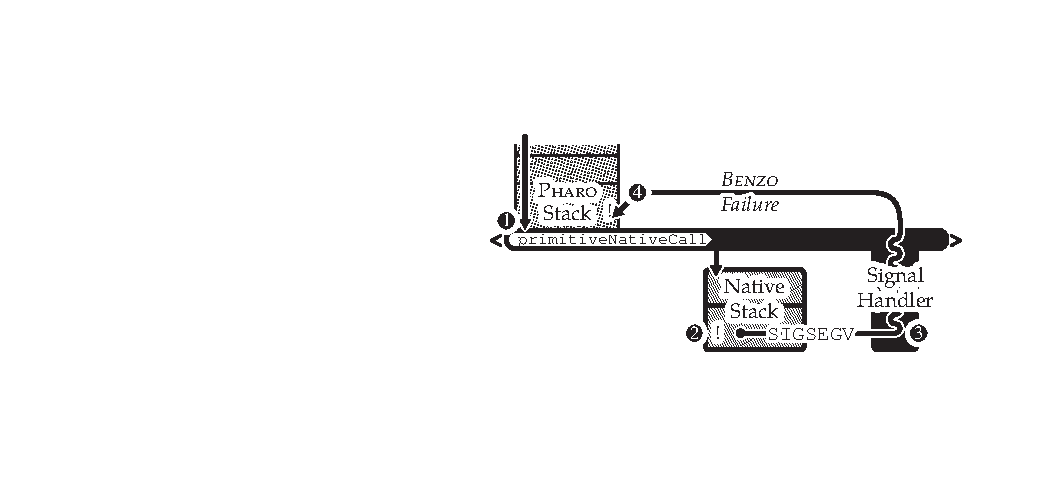
\includegraphics[scale=\imagescale]{benzo-debugger}
	\caption{\B Debugger Outline}
	\figlabel{benzo-debugger}
\end{figure}
%
\begin{enumerate}
	\item Standard \PH method activating a \B-enabled method through the \ttt{primitiveNativeCall} primitive.
	\item Native code causing a memory access violation (for example \ttt{SIGSEV}) which can not be handled by \PH directly.
	\item Low-level signal handler is activated by the operating system and tries to walk back the native stack up to the \ttt{primitiveNativeCall} activation.
	\item After successfully finding the \ttt{primitiveNativeCall} the signal handler sends a \B failure back to \PH.
\end{enumerate}

\paragraph{Barrier-free Debugging}
After proposing a solution to improve \B's bug recovery behavior we immediately encounter a second problem.
How do we debug low-level code?
With the aforementioned solution we are able to recover from certain low-level errors and signal them properly at language-side.
In a \ST-like environment the debugger will pop up on the location causing the error and thus allowing a programmer to inspect stack and variables.
To provide the same facility for \B we have to plug into the existing low-level debugging utilities such as \ttt{ptrace} to enable stepping over native instructions.

\begin{figure}[h]
	\centering
	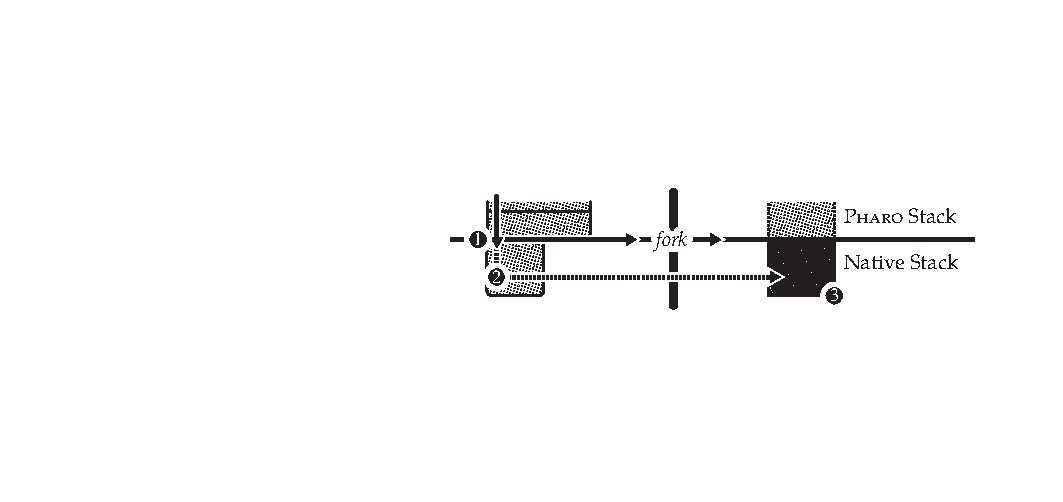
\includegraphics[scale=\imagescale]{benzo-crossover-debugger}
	\caption{\B Crossover Debugger Outline}
	\figlabel{benzo-crossover-debugger}
\end{figure}
%

\todo{ref on cross language debugger: Helvetia?}
\todo{diassembler support ...}

\todo{Extend debugging to low-level => CPU platform specific debugger necessary} \\
\todo{might be simplified by having a common infrastructure => follow up on VCPU}

% -----------------------------------------------------------------------------
\subsection{Virtual \CPU an Assembler \DSL}
% -----------------------------------------------------------------------------
\todo{small summary of the current shortcomings} \\
\todo{Current State of the Implementation} \\
\todo{Support new Platforms} \\
\todo{Indirect support for simluation and thus better debugging}


% =============================================================================
\section{\VM-level Improvements}
\seclabel{future-vm}
% =============================================================================
\todo{Introduction: Lanugage-side is not enough} \\
\todo{Need to get a onstacle-free VM} \\
\todo{List of requirements for a new VM Infrastructure} \\ 
\todo{Small comparison against the current solution we have with COG} \\


% -----------------------------------------------------------------------------
\subsection{VM-level Reification}
% -----------------------------------------------------------------------------
\todo{Resulting from the first law of Inspectors, all VM-level objects are reified} \\
\todo{List of typical objects that don't have a reification in COG} \\
\todo{List advantages}\\
\todo{make concepts explicit and first-class} \\
\todo{limit the use of raw memory access and string-based programming} \\

% -----------------------------------------------------------------------------
\subsection{Runtime Reification / Dual Objects}
% -----------------------------------------------------------------------------
\todo{Reuse the same objects for the bootstrap and at runtime inspectors/mirrors} \\
\todo{goes further than the sheer compile-time reification} \\
\todo{accessible from language-side => leads to the following MOP}

% -----------------------------------------------------------------------------
\subsection{Mate Object Model and Runtime MOP}
% -----------------------------------------------------------------------------
\todo{consequence of the runtime reification of the VM introspection => intercession}\\
\todo{Rough Overview of all the Objects currently present in Mate (UMLish)}

% -----------------------------------------------------------------------------
\subsection{Be Native}
% -----------------------------------------------------------------------------
\todo{out of the intercession capabilities follows that we need native support at runtime (see \B)}\\
\todo{that means we need to have decent / better infrasrtucture for native code}\\
\todo{need to be able to achieve what \NBJ didn't manage: compile native methods and hand them over to the \VM}\\
\todo{step towards our implementation in \Mate}


% =============================================================================
\section{\Mate a \VM prototype}
\seclabel{mate}
% =============================================================================

\begin{figure*}[h]
	\begin{adjustwidth}{-10.0in}{-10.0in}
		\centering
		
\includegraphics[width=1.02\textwidth]{mate-logo}
	\end{adjustwidth}
\end{figure*}

\todo{introduction: protoype based on the conclusions presented in the previous sections}\\
\todo{for reasearch mainly but possible long term solution to our \VM problems}

% -----------------------------------------------------------------------------
\subsection{Mate Compiler Outline}
\seclabel{future-mate-compiler}
% -----------------------------------------------------------------------------
\todo{Small Intro: Reuse the bootstrap infrastrucutre at runtime (FFI, JIT...)}

\begin{figure}[H]
\centering
	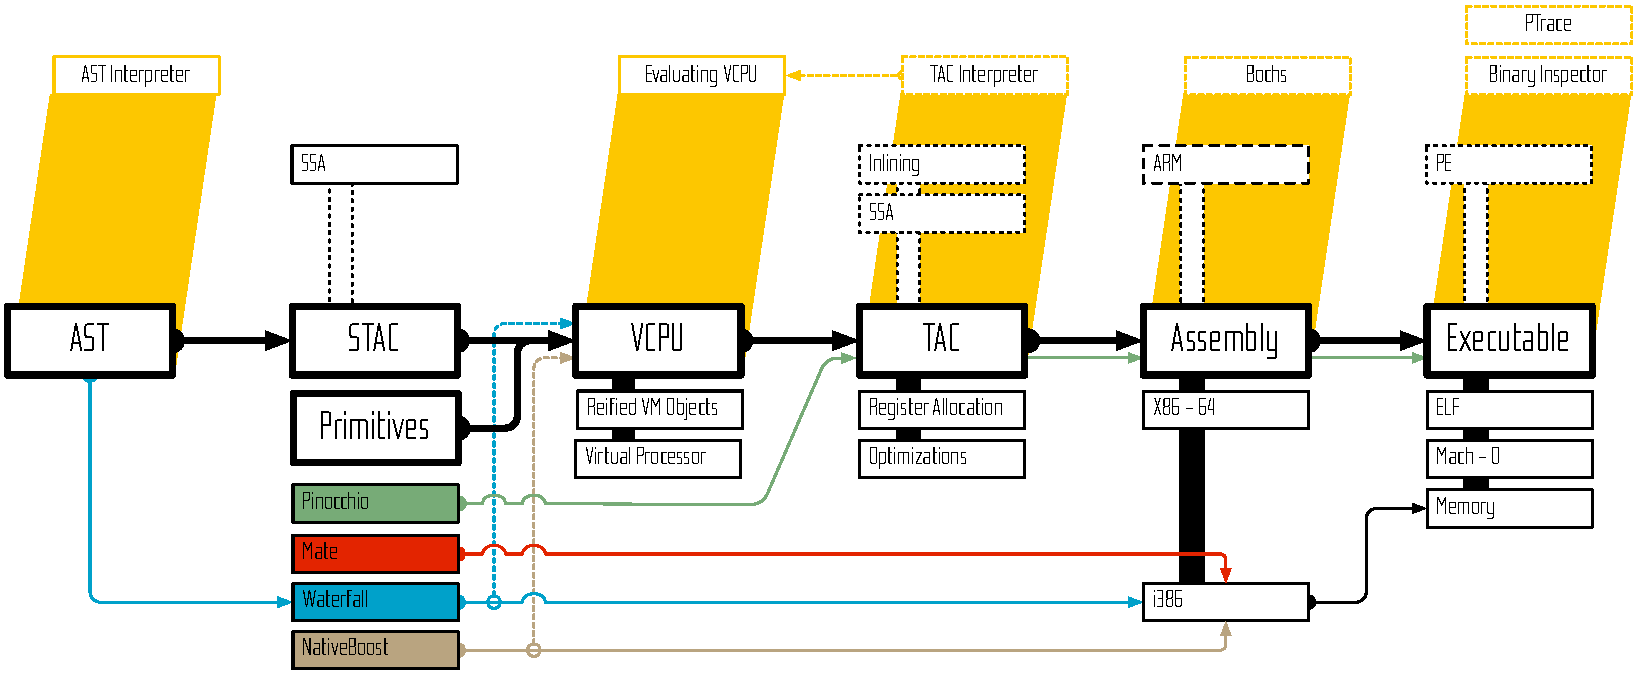
\includegraphics[width=\textwidth]{mate-compilation-toolchain}
\end{figure}

% -----------------------------------------------------------------------------
\subsection{Mate Bootstrap Outline}
\todo{Small Intro: Why Bootstrap and how to use the reified objects}\\
\todo{Compare to Pinocchio (manual approach)}\\
\todo{Work in Progress: Envision the trace-based Bootstrap}


% -----------------------------------------------------------------------------
\subsection{Mate Towards Complete Reflection}
\todo{list possible paths between the 4 quadrants of reflection}\\
\todo{usecase: dynamic gc change}\\
\todo{usecase: dynamic object format influence}\\
\todo{usecase: optimize partial behavior reflection (immutability, proxies)}\\

% -----------------------------------------------------------------------------
\subsection{Related Work}
% -----------------------------------------------------------------------------
\todo{Squeak VM} \\
\todo{Cog} \\
\todo{Pinocchio} \\
\todo{MIST}

% =============================================================================
\section{SISTA}
% =============================================================================

\todo{do we put this in a separate section?}\\
\todo{related to \NBJ, but more real-world approach}

% =============================================================================
\section{Reflective Future}
% =============================================================================
% NEW concepts
\todo{Check with GUIDO} \\
\todo{List 3 to 4 different Examples entering the 4th quadrant:}

% -----------------------------------------------------------------------------
\subsection{Accessible VM Components}
% -----------------------------------------------------------------------------
\todo{Access GC Statistics} \\
\todo{Access JIT Statistics for Type Annotations / Tooling}

% -----------------------------------------------------------------------------
\subsection{Interchangeable VM Components}
% -----------------------------------------------------------------------------
\todo{Change GC strategy} \\
\todo{Change JIT Strategy}

% -----------------------------------------------------------------------------
\subsection{Interchangeable Language Semantics}
% -----------------------------------------------------------------------------
\todo{Up to which extent can this be supported?} \\
\todo{Related to VM MOP: How much should be changeable? When?}


% -----------------------------------------------------------------------------
\subsection{Efficient Reflection}
% -----------------------------------------------------------------------------
\todo{Reflectivity at VM-level} \\
\todo{Flatten but don't freeze Reflection/Abstraction}


% =============================================================================
\section{Summary}
% =============================================================================

\todo{a lot of work on the engineering level to get a \VM with reflective properties}\\
\todo{- limited resources focused on maintaining the current infrastructure} \\
\todo{for research we have already sufficient tools at hand to experiment} \\
\todo{- outline some stuff for guido} \\
\todo{possiblity to split up off tools to be used by \PH} \\
\todo{- VCPU IR} \\
\todo{- improved FFI}


% =============================================================================
\ifx\wholebook\relax\else
    \end{document}
\fi